% cartilha-laps-semg.tex
%

\documentclass[a4paper,11pt]{article}

%=== preambulo === 
\usepackage[brazilian]{babel}
\usepackage{color,enumerate}
\usepackage[brazilian]{babel}
\usepackage{color,enumerate}
\usepackage{graphicx}
\usepackage[toc,page]{appendix}
\usepackage[table]{xcolor}
\usepackage{booktabs}
\usepackage[T1]{fontenc}
\usepackage[utf8]{inputenc}
\usepackage{subfigure}
\usepackage{fullpage}
\usepackage[backend=biber, style=authoryear, doi=false, isbn=false, url=false]{biblatex}
\addbibresource{bib/semg.bib}

%\usepackage[backref=true, pdfborder= {0 0 0}, citecolor=black, urlcolor=black, linkcolor=black, colorlinks=true]{hyperref}
%\usepackage[final]{pdfpages}
%\definecolor{lightgray}{gray}{0.9}
%\definecolor{lightblue}{RGB}{153,204,255}
%\definecolor{lightgreen}{RGB}{204,255,229}
%%\definecolor{lightyellow}{RGB}{255,255,153}
%\definecolor{lgray}{gray}{0.7}
% === ===

\title{Aquisição de sinais de eletromiografia de superfície\footnote{Este material é baseado no Trabalho de Conclusão de Curso ``Desenvolvimento e análise de protótpos para aquisição de sinal mioelétrico de superfície'', de autoria de Sérgio de Nazaré Rodrigues Lima Júnior em agosto de 2019, como requisito para obtenção do grau de Engenheiro de Telecomunicações.}}
       
\author{Grupo de análise de movimento do LaPS\\
        (LaPS/ITEC/UFPA)}
\date{Março de 2020} 


\begin{document}
\maketitle

% ======
\section{Introdução}
\label{sec:intro}
A eletromiografia é um dos recursos mais utilizados no diagnóstico e tratamento de pacientes com problemas musculares, sendo muito solicitada por ser um procedimento simples e seguro. Também é extremamente eficaz para a identificação de doenças que afetam as células nervosas ou os nervos periféricos~\parencite{MIOTEC2019}. Inumeras são as áreas onde a eletromiografia é utilizada:
\begin{itemize}
   \item Na medicina, identificando disfunções musculares de pacientes além de diagnosticar possíveis doenças graves que atigem os nervos e músculos;
   \item Na odontologia, trabalhando a região muscular da articulação mandibular;
   \item Na fonoaudiologia, com a avaliação do tratamento dos músculos pertencentes ao processo da fala;
   \item Na fisioterapia com a avaliação do potencial de resposta das celulas musculares;
   \item Na educação física, avaliando as condições dos músculos, prevenindo lesões e aplicando programa de exercícios mais adequado.
   \item No desenvolvimento de próteses interativas de membros (mãos, braços e pernas), sistemas de locomoção (cadeira de rodas), etc.
\end{itemize}
% ======

% ======
\section{Características dos sinais de SEMG}
\label{sec:carac}
O sinal mioelétrico possui duas características principais: amplitude e faixa de frequência.

A amplitude do sinal muscular varia em torno de $0$~V a $10$~mV, demandando cautela na etapa de sua aquisição, uma vez que tal amplitude é equiparável à do ruído. %devido aos possíveis ruídos em que a aquisição fica suscetível dada a pequena amplitude do sinal muscular.

A região de frequência onde a energia do sinal se concentra está entre $0$~Hz e $500$~Hz, sendo predominante no intervalo entre $50$~Hz e $150$~Hz~\parencite{DELUCA2002}.

A Figura~\ref{fig:fft_emg} apresenta um exemplo de sinal muscular, obtido pelo monitoramento da contração do músculo tibial anterior de um indivívuo. São exibidos tanto o registro temporal quando no domíno da  frequência.

\begin{figure}[h]
  \centering
  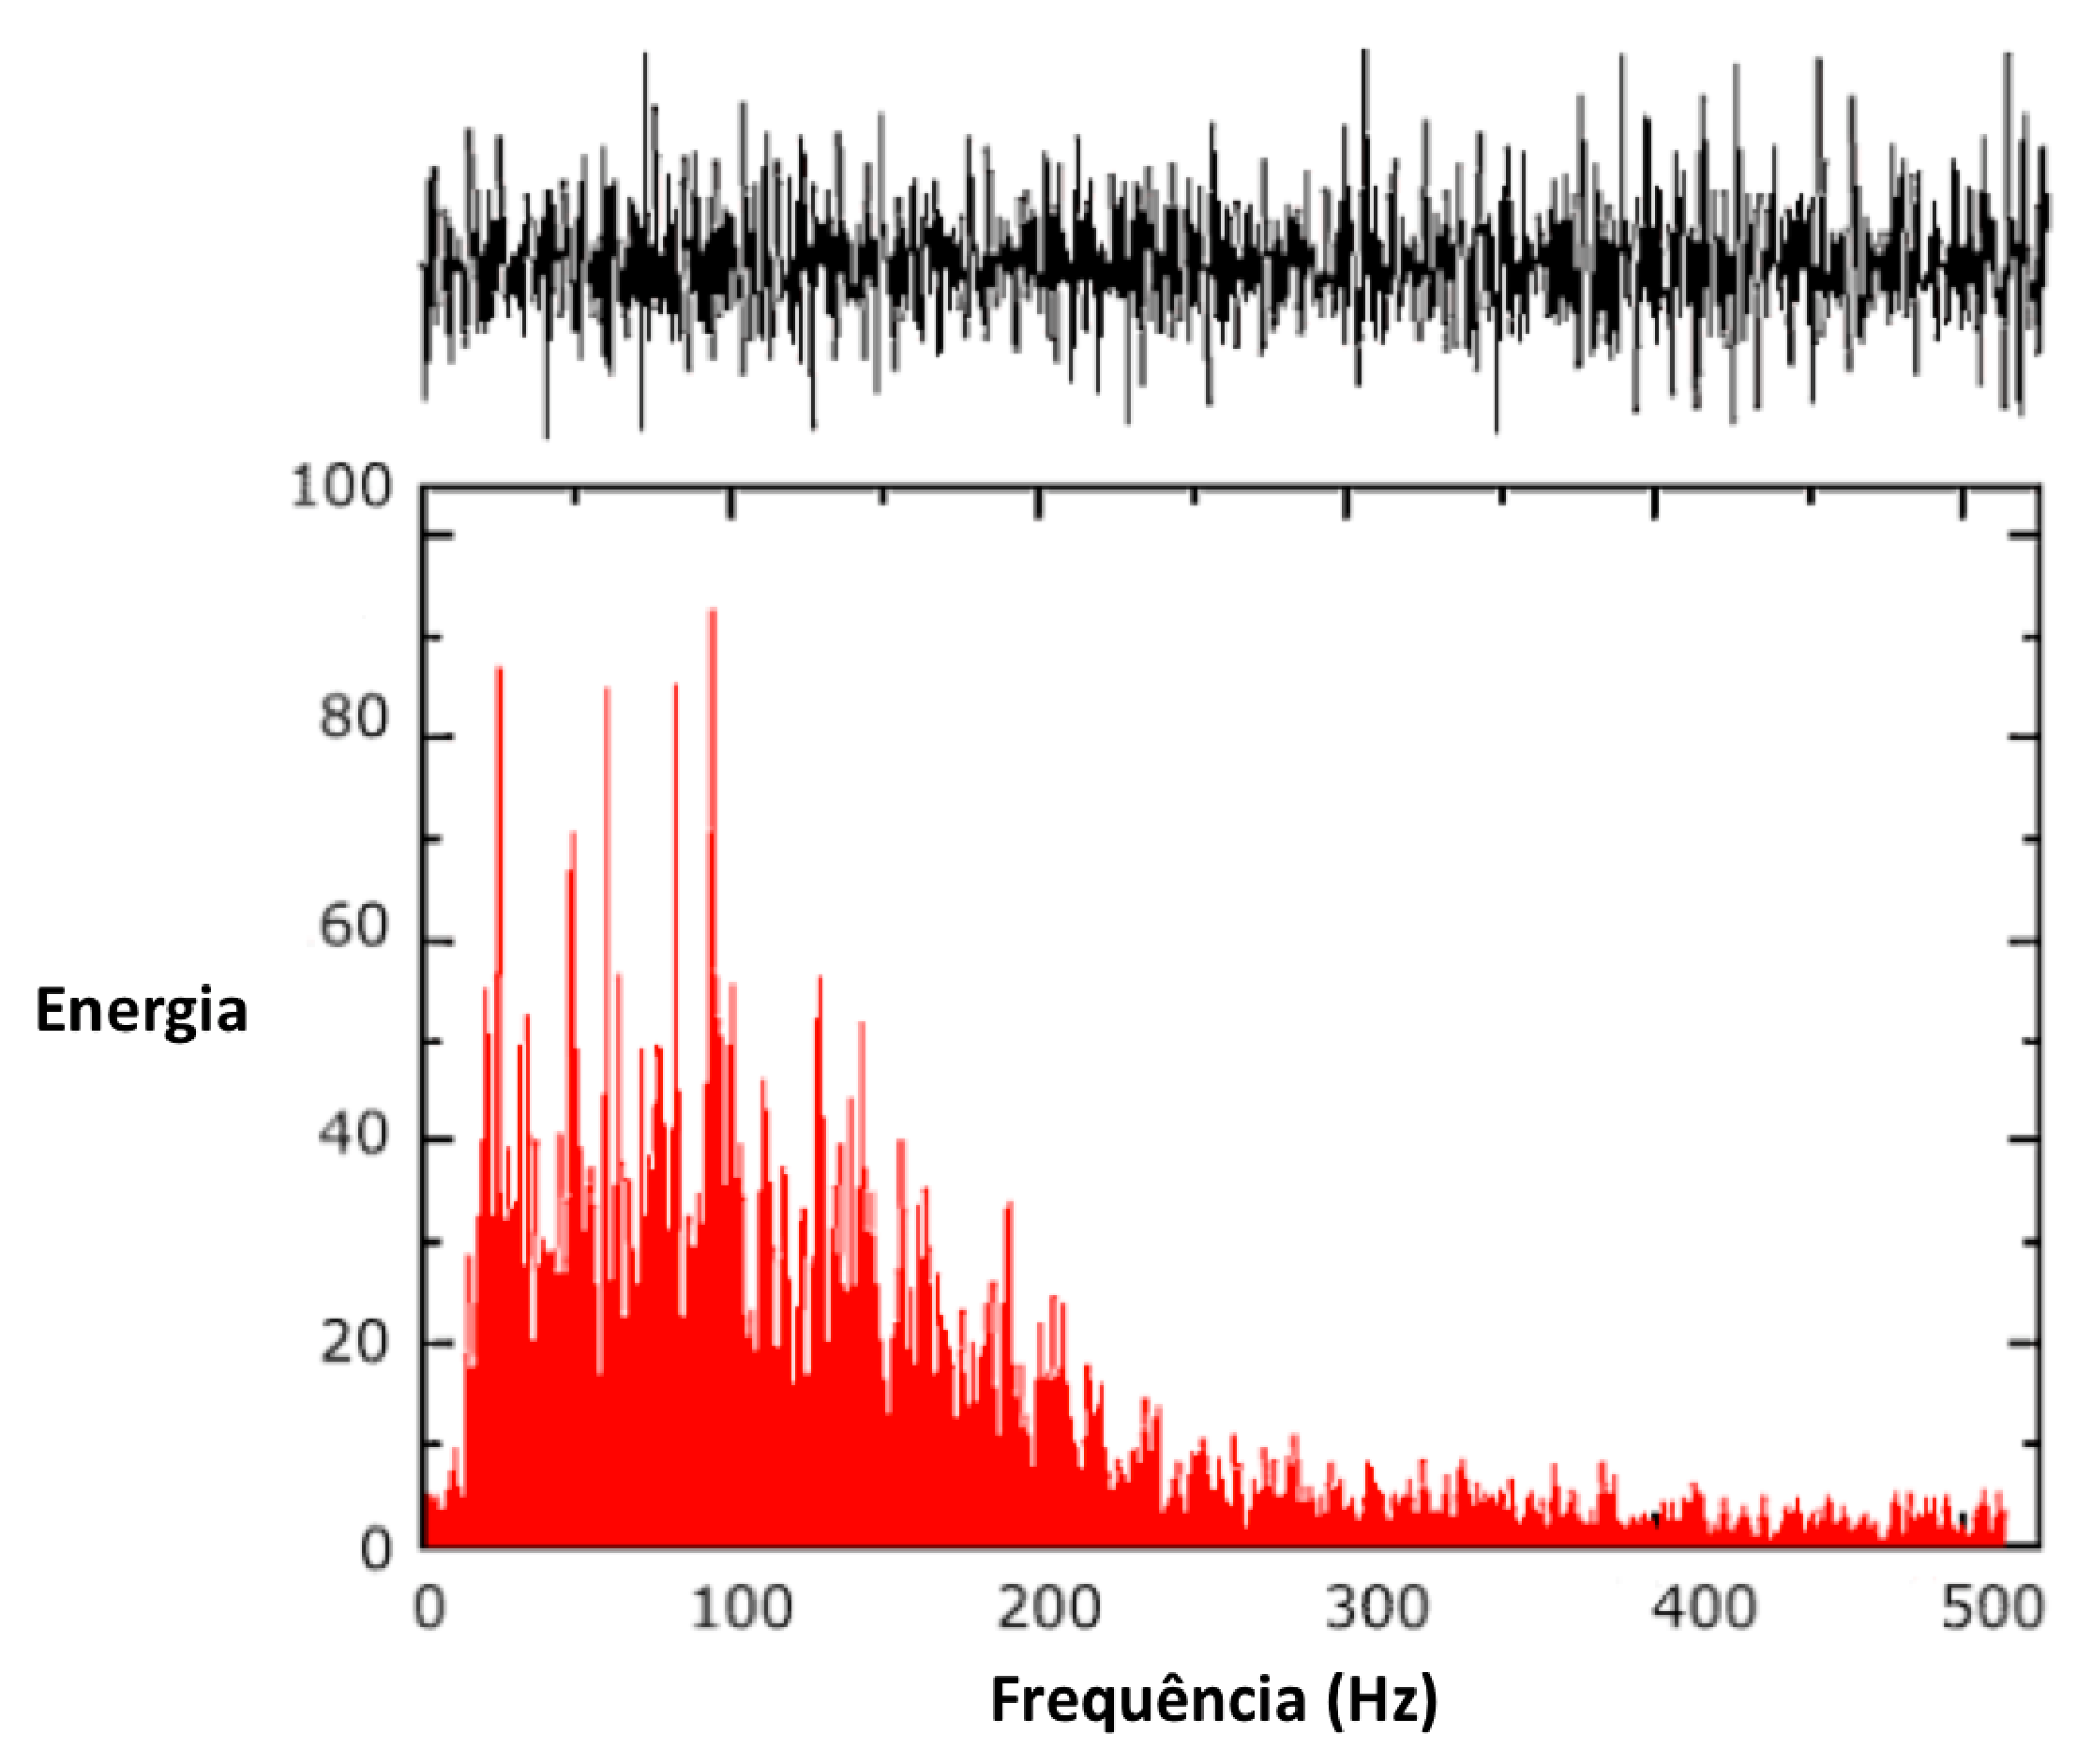
\includegraphics[scale=0.25]{fig/fft_emg.eps}
	\caption {Sinal do músculo tibial anterior nos domínios do tempo (em preto) e da frequência (em vermelho). Fonte:~\parencite{DELUCA2002}}
  \label{fig:fft_emg}
\end{figure}

Uma das principais preocupações durante a aquisição do sinal mioelétrico é com relação ao ruído presente no sinal. Diversas são as fontes típicas de ruído neste tipo de aplicação, dentre as quais:

\begin{itemize}
  \item \textbf{Ruído proveniente dos  componentes eletrônicos do circuito de aquisição:} todos os componentes eletrônicos geram ruídos que estão contidos em uma ampla faixa de frequência e que não podem ser eliminados completamente, apenas mitigados com a utilização de componentes eletrônicos de boa qualidade, elaboração cuidadosa de projeto de circuito e técnicas de construção adequadas;
  \item \textbf{Ruído ambiente advindo de fontes de radiação eletromagnética:} este tipo de ruído tem origem em lâmpadas, transmissores de rádio e televisão, fios elétricos, etc. Pode ser atenuado com a utilização de caixas metálicas para a proteção dos circuitos de aquisição;
  \item \textbf{Ruído da rede elétrica:} é o ruído de maior predominância no sinal de interesse, causado pela rede elétrica que tem como frequência fundamental $60$~Hz. Esse tipo de ruído pode ser atenuado com o uso de filtros \textit{notch} que são filtros com uma seletividade de banda de frequência muito restrita. 
  \item \textbf{Ruído de artefato de movimento:} trata-se do ruído gerado pelo movimento dos cabos que ligam os eletrodos ao circuito de aquisição e o próprio movimento entre eletrodo e a pele. Esse tipo de ruído pode ser combatido com a utilização de filtros passa-altas.
\end{itemize}
 
\section{Sistema de aquisição desenvolvido}
\label{sec:sist}
  
\section{Conclusão}
\label{sec:concl}
 
\printbibliography
\end{document}
